\chapter{Multiple Defect Diagnosis}
\label{chap:multi}

The TRAX fault model presented in Chapter~\ref{chap:trax} is designed to capture the arbitrary slowdown exhibited by only a single early-life or wear-out defect.
%
However, it is likely that more than one defect will be present, due to the very nature of the these targeted defect types.
%
For example, circuit aging (such as NBTI) will affect many PMOS transistors in a circuit, depending on the time that they are switched on by an appropriate gate voltage.
%
Also, early-life defects caused by fabrication process variation are likely to occur in clusters based on that variation, leading to a circuit affected by multiple defects.
%
With the conservative propagation properties of the unknown value \textit{X}, the use of a TRAX-based fault dictionary can remain effective even in the presence of multiple defects.
%
This is especially true with the relaxed diagnostic requirements of on-chip diagnosis (that is, fault localization only to the level of repair, replacement, or avoidance).
%
The objective of this chapter is to perform an analysis of the effectiveness of the TRAX-based hierarchical fault dictionary for on-chip diagnosis when diagnosing the response of multiple defects due to ELF and/or wear-out.


\section{Defect Injection Sites}
\label{sec:multi_defect_injection_sites}

In Section~\ref{sec:multi_experiments}, a variety of defect injection experiments are performed.
%
For each experiment, several (virtual) delay defects are injected into a circuit, a set of test pairs are simulated, and the circuit simulation response is evaluated for correctness.
%
Any failing tests are used with the fault dictionary to determine the likely defective modules.
%
This procedure is very similar to the defect injections and diagnosis experiments of Section~\ref{sec:diag_exp_diag}, however, there are two important differences explained next.

First, multiple (virtual) delay defects are injected into the circuit.
%
A critical aspect of the multiple defect injection experiments is defect site selection.
%
To provide the most realistic defect injection experiments, the distribution of injected defects should reflect the distribution of the targeted defects (namely, early-life and wear-out defects).
%
Additionally, randomized defect injection experiments are performed to provide a comparison.
%
Second, the delays injected for multiple defect injection experiments are set to the single-defect delay from Section~\ref{sec:diag_exp_diag}, and do not change during the course of the experiment.

\subsection{Defect distribution: Random}
The most straight-forward approach for defect injection is a random selection of defect sites.
%
This provides a comparison with the more-targeted, locality- and usage-based defect injection experiments described next.
%
Additionally, random defect injection provides an analysis for randomly-distributed failures.
%
To perform a random defect injection experiment, $k$ random gates and polarities (STF or STR) are selected (without replacement).
%
For each selected gate and polarity, the corresponding pre-computed TRAX delay (either a rising delay or falling delay) is added to the corresponding rising/falling delay of the selected gate using a testbench-level gate parameter override.
%
The randomly-selected defects may belong to multiple different recovery-level modules, increasing the difficulty of on-chip diagnosis.

\subsection{Defect distribution: Locality-based}
Early-life failures such as gate oxide defects are caused by fabrication defects due to natural variation in the IC fabrication process~\cite{chen08}.
%
If process variation creates a gate oxide defect at a particular location, we are likely to find other gate oxide defects in close proximity, because such variation typically exhibits spatial correlation~\cite{agarwal03}.
%
Spatial correlation is the phenomenon where transistors close to each other are likely to have similar characteristics~\cite{xiong07}.
%
Locality-based defect injection attempts to emulate this trend for some defects (those caused by process variation) to be more likely located nearby.
%
The goal here is not to try to realistically model process variation, but to instead model the spatial locality relationships of randomly-selected defects.

To accomplish this, a commercial place-and-route tool is used with each circuit to estimate the approximate coordinate positions of each gate within the design placement.
%
An example placement for benchmark circuit c7552~\cite{brglez85} is shown in Figure~\ref{fig:multi_gate_placement_c7552}.

%\vskip 0.5em%
\begin{figure}[hbtp]
\centering
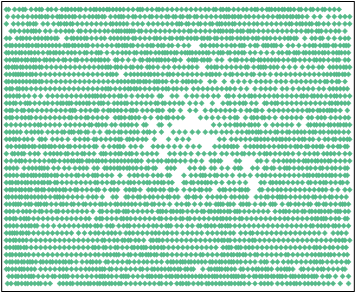
\includegraphics[width=0.5\columnwidth]{fig_multi_gate_placement_c7552}
\caption{Gate placement created by a commercial place-and-route tool for benchmark circuit c7552~\cite{brglez85}.}
\label{fig:multi_gate_placement_c7552}
\end{figure}
%\vskip 0.5em%

The list of gate placement coordinates is transformed into a sorted list of the nearest neighbors for each gate.
%
To perform a locality-based defect injection experiment, a random gate and defect polarity (STF or STR) are selected along with the nearest neighbors of the selected gate.
%
For each selected defect, the corresponding pre-computed TRAX delay (either a rising delay or falling delay) is added to the corresponding rising/falling delay of the selected gate using a testbench-level gate parameter override.
%
As already mentioned, the selected defects may belong to multiple recovery-level modules.

The simplistic approach used here differs from more advanced approaches such as~\cite{cai16}, where process variation is modeled in a hierarchical fashion, based on the work in~\cite{xiong07}.
%
In these approaches, the variation of an individual transistor is modeled as the sum of a hierarchy of random variables at the die level, the core level, and core-component level.
%
Modeling process variation at each level significantly reduces the complexity of analyzing spatially-correlated dependent random variables.
%
Such models require real-world measurements of IC variation, which can be accomplished using arrays of ring oscillators~\cite{bushan06} or by recording and analyzing near-infrared light emissions~\cite{stellari09}.
%
The approach presented here could be enhanced to receive input from such models and measurements to provide a more realistic selection of delay defects.
%
Further investigation of this topic is a rich area for future work.

\subsection{Defect distribution: Usage-based}
Defects induced or exacerbated by normal circuit operation, typically termed aging or wear-out defects, are targeted by usage-based defect injection.
%
For example, NBTI (negative bias temperature instability) affects the PMOS transistors of a logic gate, causing circuit speed degradation~\cite{borkar06, schroder03}.
%
While already an issue at 90nm~\cite{agarwal07}, the effects of NBTI continue to worsen as process technology continues to scales down~\cite{reddy02}.
%
The effects of NBTI increase while the PMOS transistor is turned on (has a logic-low input), and can be partially reversed while the transistor is turned off.
%
In an actual circuit, many of the PMOS transistors will become affected by NBTI during the life of the circuit.
%
However, not all affected transistors will result in an observable failure, as many of the slowdowns will affect non-critical paths and not affect any circuit output.

The ideal method of selecting defects to emulate usage-based degradation would start by tracking the usage of each PMOS transistor as the circuit is exercised with some workload.
%
Ideally, a realistic workload would be used to obtain the most accurate aging for each PMOS transistor.
%
This information would provide an estimate of the actual delay of each PMOS transistor affected by NBTI.
%
The resulting slowdowns can then be injected into the simulated circuit to determine if any failures occur.

The approach taken here differs slightly from the ideal approach.
%
To estimate usage-based transistor degradation, the TRAX fault simulator (Section~\ref{sec:trax_gpu}) is instrumented to track the number of ``ON'' cycles for the PMOS transistors in each gate.
%
Instead of a realistic workload, a test set of 100,000 random test pairs is generated and applied to each circuit using the instrumented fault simulator.
%
This results in a list of PMOS transistors potentially affected by NBTI, filtered to contain only those that spent more than 70\% of the test cycles in the ON state.
%
While this may not exactly match the transistor aging profile generated from a more realistic workload, we believe that the large number of random test vectors used provides a good characterization of the relative transistor aging in the circuit.
%
A histogram of the (unfiltered) PMOS transistor ON times for the circuit L2B~\cite{sun11} is shown in Figure~\ref{fig:multi_pmos_usage_l2b}.
%
It should be noted that any circuit workload (besides random) and threshold could be used instead of the ones chosen here.

%\vskip 0.5em%
\begin{figure}[hbtp]
\centering
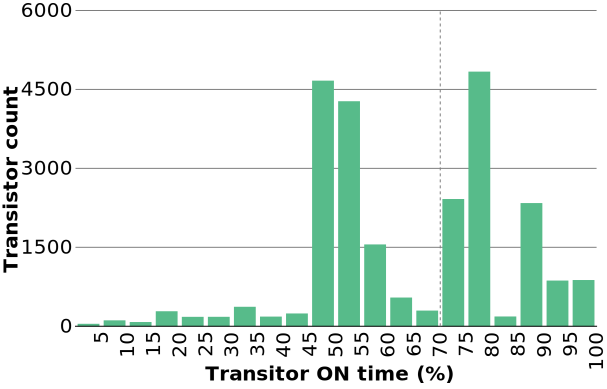
\includegraphics[width=0.8\columnwidth]{fig_multi_pmos_usage_l2b}
\caption{A histogram of the (unfiltered) PMOS transistor ON times for circuit L2B~\cite{sun11}.
%
The dashed line indicates the cutoff above-which transistors are considered NBTI-affected.}
\label{fig:multi_pmos_usage_l2b}
\end{figure}
%\vskip 0.5em%

To perform a usage-based defect injection experiment, $k$ random PMOS transistors are selected (without replacement) from the filtered set of NBTI-affected transistors\footnote{Random selection here is restricted to the set of NBTI-affected transistors, and is not a random selection of all circuit transistors.}.
%
This is slightly different from the previous two defect injection schemes.
%
Whereas random- and locality-based defect injection experiments add additional delay (either rising or falling) to a gate output, the usage-based defect injection experiments add delay only to a specific input-to-output transition for the affected gate.
%
That is, we perform transistor-level delay injection as opposed to gate-level delay injection.
%
This is accomplished through the following process.
%
For each of the $k$ random NBTI-affected transistors selected for an experiment, a custom logic gate is created, containing pin-to-pin timing specifications for the affected input transistor, based on the STR TRAX delay for that gate.
%
The STR TRAX delay is used because NBTI-affected PMOS transistors increase the gate output rise time\footnote{Care must be taken to consider how layout cell implementation may affect this assertion.
%
For example, if an AND gate is implemented by a NAND cell followed by an INV cell, the presence of extra PMOS transistors must be accounted for.}.
%
The original circuit design file is then programmatically modified to swap-in the customized gates, and gate-level simulation proceeds as normal.
%
As already described, the selected defects may belong to multiple recovery-level modules.
%
Note that in the ideal case, the aging of each PMOS transistor would determine the additional delay injected into the gate, while our experiments here use the TRAX delay (the minimum detectable delay for a fault site, empirically determined as part of the single defect injection experiments of Section~\ref{sec:diag_exp_diag}).


\section{Multiple Defect Diagnosis}
\label{sec:multi_diagnosis}
To reiterate, the end goal of on-chip diagnosis is to identify the failing modules of a core/uncore that has failed testing.
%
The result of performing each multiple-defect injection experiment described in Section~\ref{sec:multi_defect_injection_sites} is a pass/fail circuit response, consisting of one bit (pass or fail) for each applied test pair.
%
As detailed in Chapter~\ref{chap:diag}, diagnosis proceeds by analyzing the pass/fail result for each test pair in turn.
%
For each failing test, any candidate faults that are inconsistent with the test failure (that is, a Tester-Fail/Simulation-Pass situation) are eliminated from further consideration, that is, they are no-longer candidate faults.
%
Once all test responses are analyzed, the remaining candidate faults are used to generate a per-module count of candidate faults.
%
This part of the on-chip diagnosis process does not change in a multiple-defect context and remains the same as when diagnosing single defects in Section~\ref{sec:diag_exp_diag}.

As before, the per-module counts of candidate faults are used to evaluate the quality of the diagnosis result.
%
For the diagnosis experiments of Chapter~\ref{chap:diag}, where a single defect is injected for each experiment, a diagnosis result is deemed ``accurate'' if the defective module has a non-zero candidate fault count.
%
A diagnosis result is deemed ``ideal accurate'' if the defective module has the highest candidate fault count of all modules.

This evaluation process must be slightly altered when diagnosing multiple defects, because there is likely more than one defective module (i.e., a module that has one or more injected defects).
%
Here, ``accuracy'' is defined as a diagnosis result where all defective modules have non-zero candidate fault counts.
%
``Ideal accuracy'' is defined as a diagnosis result where all defective modules have candidate fault counts larger than the largest count of a non-defective module.
%
In other words, ideal accuracy occurs when no non-defective module would be placed higher than a defective module when ranked by candidate fault count.
% TODO add an image to show how this works, especially the "larger than the largest count of a non-defective module" part?

Additionally, a new ``partial accuracy'' metric is calculated for the multiple defect injection diagnosis results.
%
Whereas a single defect injection diagnosis is either inaccurate or accurate (the defective module has a zero or non-zero candidate fault count, respectively), the diagnosis result of an $n$-defect injection experiment may have from 0 through $n$ defective modules with a non-zero candidate fault count.
%
The partial accuracy metric is defined as the percentage of defective modules with non-zero candidate fault count.
%
For example, if a multiple defect injection experiment has five defective modules, a diagnosis result with all five modules having a non-zero candidate fault count would be classified as accurate with a partial accuracy of 100\%.
%
The partial accuracy metric is evaluated in addition to the existing metrics of accurate and ideal accurate, so it is possible that a 100\% partial accurate diagnosis (which would be deemed accurate) may also be ideal accurate, depending on the candidate fault counts of the non-defective modules.
%
Continuing the example, a diagnosis result with all five modules having zero candidate faults would be classified as inaccurate with a partial accuracy of 0\%.
%
Finally, a diagnosis result with, say, three of the five defective modules having a non-zero candidate fault count would be classified as inaccurate, but with a partial accuracy of 60\%.

It is entirely possible that one or more of the injected defects belong to the same module.
%
In these situations, for the purposes of computing the ``partial accuracy'' metric, the corresponding module of each injected defect is treated as an independent defective module.
%
For the example above with five injected defects, consider the situation where three of the five defects belong to module $A$, and two defects belong to module $B$.
%
With regard to ``partial accuracy,'' there are four possible scenarios.
%
First, if modules $A$ and $B$ both have zero candidate fault counts, the diagnosis result has a partial accuracy of 0\%.
%
Similarly, if both modules have non-zero candidate fault counts, the diagnosis result would have a partial accuracy of 100\%.
%
If only module $A$ has a non-zero candidate fault count, then three of the five defective modules are accurate, resulting in a partial accuracy of 60\%.
%
If only module $B$ has a non-zero candidate fault count, then two of five defective modules are accurate, leading to a partial accuracy of 40\%.
% TODO add an image to show this?

\section{Experiments}
\label{sec:multi_experiments}

Experiments are performed to evaluate the suitability of the TRAX fault model and the hierarchical dictionary for the task of diagnosing multiple injected defects.
%
Each experiment injects delay defects into a circuit and then performs gate-level simulation to determine if any incorrect responses are observed.
%
The result of this simulation is a list of pass/fail values, one for each simulated test-pair.
%
The fault dictionary is used with the pass/fail test responses to determine the set of TRAX faults that are compatible with the observed test results, that is, the presence of any of these compatible faults could explain the observed behavior.
%
Given that the end goal of TRAX on-chip diagnosis is to determine which module (or modules) are defective, the compatible faults are divided into groups based on the module where each belongs.
%
The counts of compatible faults belonging to each module are used to evaluate the quality of the diagnosis results, as explained in Section~\ref{sec:multi_diagnosis}.

The experiments presented here use c432 and c7552 from the ISCAS85 benchmark circuits~\cite{brglez85}.
%
Additionally, the L2B uncore from the OpenSPARC T2 processor design~\cite{sun11} is also used.
%
Twelve groups of defect injection experiments are performed for each of these three circuits, with 1,000 defect injections for each group.
%
The twelve groups for each circuit are divided into three groups of four (each group of four injecting 2, 5, 10, and 20 defects) for random-, locality-, and usage-based defect injections (as described in Section~\ref{sec:multi_defect_injection_sites}).

The diagnosis results for circuits c432, c7552, and L2B are shown in Figures~\ref{fig:multi_heatmap_c432}, \ref{fig:multi_heatmap_c7552}, and \ref{fig:multi_heatmap_l2b}, respectively.
%
Each figure has one column per experiment, grouped into random-, locality-, and usage-based defect injections, with 2-, 5-, 10-, and 20-injection experiments for each group.
%
The first two rows are the percent accurate (\%A) and percent ideal accurate (\%IA), followed by the partial accuracy histogram (as described in Section~\ref{sec:multi_diagnosis}).
%
Additionally, the partial accuracy histogram is shaded to highlight the larger bins, with darker background color indicating a higher percentage of diagnosis results.
%
The presence of empty (``$0.0$'') bins for the 2-, 5-, and 10-injection experiments is due to the quantization of partial accuracy, based on the number of injected defects.
%
For example, when injecting five defects the partial accuracy can have 0, 1, 2, 3, 4, or 5 modules correctly identified, corresponding to 0\%, 20\%, 40\%, 60\%, 80\%, or 100\% partial accuracy, respectively.

%\vskip 0.5em%
\begin{figure}[hbtp]
\centering
\includegraphics[width=\linewidth]{fig_multi_heatmap_c432}
\caption{Diagnosis results of multiple defect injection experiments for circuit c432.
%
Data rows labeled \%A and \%IA are the percentage of diagnosis results deemed accurate and ideal accurate, respectively.
%
The bottom row contains a small plot showing the distribution of the number of defective modules for each of the 1,000 experiments collated in the column.
%
The remaining rows are a normalized histogram of partial accuracy, shaded to highlight the larger bins.}
\label{fig:multi_heatmap_c432}
\end{figure}
%\vskip 0.5em%

%\vskip 0.5em%
\begin{figure}[hbtp]
\centering
\includegraphics[width=\linewidth]{fig_multi_heatmap_c7552}
\caption{Diagnosis results of multiple defect injection experiments for circuit c7552.
%
Data rows labeled \%A and \%IA are the percentage of diagnosis results deemed accurate and ideal accurate, respectively.
%
The remaining rows are a normalized histogram of partial accuracy, shaded to highlight the larger bins.}
\label{fig:multi_heatmap_c7552}
\end{figure}
%\vskip 0.5em%

%\vskip 0.5em%
\begin{figure}[hbtp]
\centering
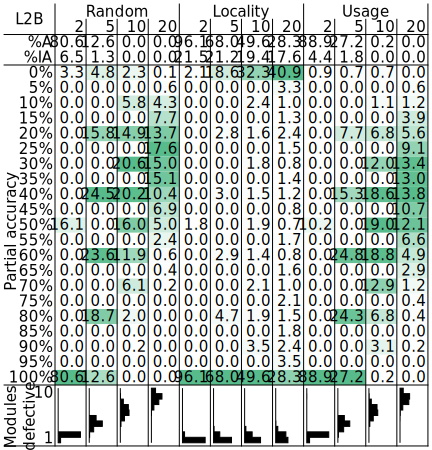
\includegraphics[width=\linewidth]{fig_multi_heatmap_l2b}
\caption{Diagnosis results of multiple defect injection experiments for circuit L2B.
%
Data rows labeled \%A and \%IA are the percentage of diagnosis results deemed accurate and ideal accurate, respectively.
%
The remaining rows are a normalized histogram of partial accuracy, shaded to highlight the larger bins.}
\label{fig:multi_heatmap_l2b}
\end{figure}
%\vskip 0.5em%

Below the partial accuracy histogram is a small plot showing the distribution of the number of defective modules for each of the 1,000 experiments collated in the column.
%
Due to the random selection of defects for injection, it is not guaranteed that all selected defects will be in separate modules.
%
Additionally, for the locality- and usage-based defect selection, it is expected that many of the selected defects will lie within the same module.
%
The maximum number of defective modules is the smaller of the number of modules in the circuit and the number of injected defects.
%
For example, each column of 2-injected defects has either one or two defective modules.
%
The defective module count plots reveal that for random defect selection, the number of defective modules also increases with the number of defects.
%
For the locality-based defect selection, there are fewer defective modules, meaning that the injected defects belong to the same few modules instead of being distributed throughout all modules.
%
The usage-based defect selection experiments show a defective module count distribution similar to the random experiments, but with a slightly smaller number of defective modules.

In general, the diagnosis results show better results for fewer defect injections (columns corresponding to 2- and 5-defect injections).
%
As more defects are injected, the partial accuracy histogram shows a shift from higher to lower partial accuracy.
%
Altogether, it appears that this approach is ineffective at diagnosing more than two delay defects.
%
However, it is important to note that the CASP on-chip test process~\cite{li08} uses periodic self-test with accelerated test conditions, in an effort to detect these gradual slowdowns before they affect correct system operation.
%
The periodic self-test will detect each defect as soon as it degrades sufficiently to produce incorrect output during the accelerated test, so ideally there will be only a few concurrent defects, maximizing the diagnostic ability of the TRAX fault model and hierarchical dictionary.

Comparisons are also drawn between the diagnosis results for random-, locality-, and usage-based defect selection.
%
For all three circuits analyzed, the diagnosis results for the locality-based defect injection experiments are more promising than the random- or usage-based experiments.
%
This is because gates in the same hierarchical module are likely to be placed in close proximity by the place-and-route tool to minimize wiring distances, logically leading to more injected defects belonging to the same module.
%
When many injected defects lie within the same module, it is likely that more candidate faults will belong to that defective module, increasing the diagnosis quality.

The diagnosis results for the usage-based defect injection experiments for c432 bear further analysis.
%
As shown in the rightmost four columns of Figure~\ref{fig:multi_heatmap_c432}, the diagnosis results are entirely bimodal, with each diagnosis result being either 0\% partially accurate or 100\% partially accurate.
%
When analyzing the most-aged PMOS transistors (based on transistor ON time during test application, details in Section~\ref{sec:multi_defect_injection_sites}), it happened to be that the top 30\% most-aged transistors are all located within the same module.
%
This is possibly due to the relatively smaller size of this circuit (208 gates), as this behavior is not observed for either of the other two circuits.


\subsection{Interaction of Multiple TRAX Faults}
The experiments presented here are an evaluation of the ability of the un-modified TRAX fault model and hierarchical fault dictionary to diagnose the response of multiple injected defects.
%
Another potential approach to this problem might involve modifying the diagnosis process and on-chip diagnosis architecture to better encompass the fault effects of multiple defects.
%
Here, we analyze the efficacy of the TRAX-based dictionary for the diagnosis of multiple delay defects, each of which is modeled by a TRAX fault.
%
Specifically, the interaction of fault effects (i.e., unknown values \textit{X}) from more than one activated TRAX fault is analyzed.

Due to the conservative propagation of the faulty \textit{X} value, a TRAX fault response subsumes any possible response of a co-located delay defect.
%
That is, the observed response of any defect must be a subset of the corresponding TRAX fault response, and it is not expected to be an exact match.
%
This is the basis of the TFSP diagnosis process outlined before, where an observed test failure will eliminate any modeled faults that could not have produced a failure for that test.

The combined response of two or more TRAX faults is simply the union of the failing values (due to the non-destructive and non-masking interactions of \textit{X} values).
%
However, unlike the single defect situation, where the defect response must be a subset of the corresponding TRAX fault response, the situation is more complex when analyzing the response of multiple defects.
%
No assumptions are made about which TRAX faulty outputs will fail due to the presence of the corresponding defects.
%
Because of this, it is possible that the defective circuit will fail any combination of the potentially failing tests from the union of TRAX fault responses.
%
This may result in a defective circuit test response, that when used with the TFSP-based on-chip diagnosis, eliminates all candidate faults due to the test response being incompatible with all modeled faults.

%\vskip 0.5em%
\begin{table}[hbtp]
\centering
\begin{tabular*}{0.9\columnwidth}{@{\extracolsep{\fill}}cccccccl}
\toprule
Fault&Module&$T_1$&$T_2$&$T_3$&$T_4$&$T_5$&\\
\midrule
$F_1$&$M_1$&P&F&F&P&F&\\
$F_2$&$M_1$&P&F&F&P&F&Eliminated (EQU)\\
$F_3$&$M_1$&P&F&P&P&P&Eliminated (SUB)\\
$F_4$&$M_1$&F&F&P&P&F&\\
\midrule
$F_5$&$M_2$&F&F&P&P&F&\\
$F_6$&$M_2$&P&P&F&F&P&\\
\bottomrule
\end{tabular*}
\caption{TRAX fault dictionary data illustrates dictionary compaction, using equivalence and subsumption relationships to eliminate two intra-module faults.}
\label{table:multi_fault_resp}
\end{table}
%\vskip 0.2em%

As an example, consider two faults from Table~\ref{table:multi_fault_resp}, $F_1$ and $F_4$.
%
These faults belong to the same module, and because they are not equivalent and neither subsumes the other, the dictionary compaction process does not eliminate either.
%
Their pass/fail responses (represented by `P' and `F', respectively, in the table rows) show at least one test where one fault could produce a failure and the other fault could not (i.e., $F_1$ uniquely fails $T_3$, and $F_4$ uniquely fails $T_1$).
%
For example, if a circuit is affected by defects at the same locations as $F_1$ and $F_4$, testing might produce a test response of ``PFPPF'', ``FPPPF'', or ``FFFPP'', among other possible test responses.
%
Diagnosing the third possible test response ``FFFPP'', the first failure would eliminate $F_1$ as a candidate fault, and the third failure would eliminate $F_4$, due to a Tester-Fail/Simulation-Pass (TFSP) condition for both faults.

Again, given the conservative propagation properties of the unknown value \textit{X}, the set of failing outputs is only a ``worst case'' accounting of the fault response.
%
The actual set of failing circuit outputs and failing tests will likely be much smaller, enabling accurate diagnosis of multiple failures, as demonstrated in Section~\ref{sec:multi_experiments}.
%
The use of such an approach, where multiple TRAX faults are merged and stored in the dictionary, deserves further investigation.
%
However, the approach may suffer from a much larger dictionary due to the $n \times (n - 1)$ fault pairs modeled.
%
Alternatively, modifications might be made to the diagnosis architecture to perform the TRAX fault effect merging during diagnosis.


\section{Summary}
\label{sec:multi_summary}

While the experiments of Section~\ref{sec:diag_exp_diag} performed single-defect injection diagnosis, a natural extension of that work is to consider how well on-chip diagnosis performs with a circuit that is affected by multiple defects.
%
The hypothesis here is to see if the TRAX fault model, the hierarchical dictionary, and the on-chip diagnosis process is similarly effective at localizing defects to the recovery-level module(s).
%
To provide for more realistic multiple-defect injection experiments, three defect selection approaches are developed, including a simple random selection, plus a locality-based defect selection process targeting gate oxide defects, and a usage-based defect selection process targeting NBTI slowdown defects.
%
These three approaches (random, locality, usage) are used to perform over 30,000 multiple defect injection experiments.

The results of the defect injection experiments are diagnosed by the on-chip diagnosis process, using a standard TRAX hierarchical fault dictionary.
%
While the first half of the on-chip diagnosis process (using occurrences of Tester-Pass/Simulation-Fail (TPSF) to eliminate faults from further consideration) remains the same, the diagnosis evaluation metrics of ``accuracy'' and ``ideal accuracy'' are updated to work in the context of multiple defective modules.
%
For example, a diagnosis result where all defective modules have non-zero candidate fault counts would be deemed accurate.
%
Additionally, a partial-accuracy metric is also developed to provide a measure of accuracies between 0\% and 100\% accurate.
%
Diagnosis results typically achieve more than 90\% accuracy when diagnosing two injected defects, with especially promising results for locality-based defect injection.
%
Altogether, the TRAX fault model, the hierarchical dictionary, and on-chip diagnosis are shown to be an effective tool for diagnosing two concurrent defects.
%
It is possible, however, to improve on these results by developing an approach that directly analyzes the effects of multiple defects.

